% !Rnw root = main.Rnw
\noindent In the first session we we will define our \textbf{\emph{mission}} and evaluate why R is the tool of choice that enables us to achieve our mission. Moreover, we will present an overview of the \textbf{\emph{concepts}} for programming with R. Then we will introduce the ``R environment'' and provide instructions for setting up \textbf{\emph{RStudio}}. Furthermore, we will explain different features of the RStudio environment so that the reader gets accustomed to working with RStudio. Finally, we will demonstrate how to read data sets, organized in tabular format, into R and take the first steps towards processing and transforming such data.
Throughout this manual, the participant will come across the following two icons

\begin{DIY}{Think}
\emph{This icon urges the reader to think about the question that has been asked and such questions will be the main discussion points during sessions.}
\end{DIY}

\begin{DIY}{Homework}
\emph{This icon will be associated with an assignment and the participants are expected to work on these.}
\end{DIY}

\begin{DIY}{Warning}
\emph{This icon will be used when we want the reader to pay attention to a particular idea.}
\end{DIY}


\vspace{\baselineskip}
\vspace{\baselineskip}
\vspace{\baselineskip}
\begin{DIY}{Think}
Why has this session been titled \textbf{``The Liftoff''}?
\end{DIY}


\clearpage

% !Rnw root = Introduction.Rnw
%==============================
\section{The Mission}
%==============================
\begin{HIGHLIGHT}
\par\noindent{
{\centering\textbf{\emph{\Huge ``Data Exploration''}} \\}
\vspace{\baselineskip}
\textbf{Data Exploration} entails the following actvities:
\begin{enumerate}
      \item Formulation of  meaningful questions
      \item Organization of data in a way to answer the questions
\end{enumerate}
}
\end{HIGHLIGHT}

\begin{DIY}{Homework}
\emph{Explore} the dataset in exercise1.csv
\end{DIY}
%=============================
\subsection{Data and Society}
%=============================
\begin{figure}[ht]
 \centering
    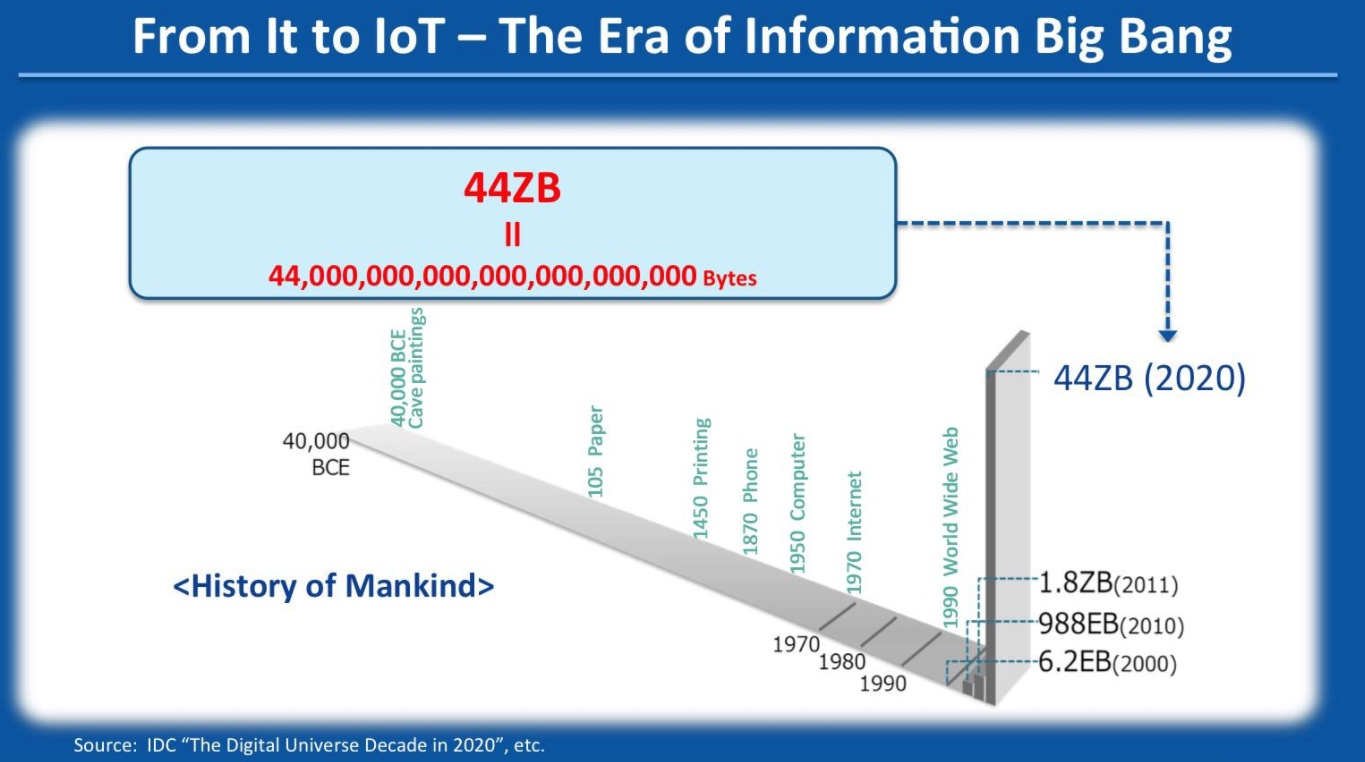
\includegraphics[width = 10 cm]{./viz/ext/DataVolumesVSHumanHistory.jpeg}
\end{figure}

\begin{DIY}{Think}
It is true that data is ubiqutous to modern society and is being generated at an unprecedented scale at high \textbf{\emph{volumes}}, \textbf{\emph{velocity}} and \textbf{\emph{variety}} (the \textbf{3V's}). Try categorizing each of the data source in the infographic ``\emph{Data Never Sleeps 5.0}''
\begin{itemize}
  \item into one of the \textbf{3V's}  
  \item \textbf{\emph{high noise-to-signal}} ratio source v/s \textbf{\emph{low noise-to-signal}} ratio source
  \item sources where high volume \textbf{\emph{correlates}} to better insights 
\end{itemize}
\end{DIY}

\begin{DIY}{Homework}
Read Section 19 of the \emph{Statistical Analysis Handbook}
\end{DIY}

\begin{DIY}{Think}
Argue why the \textbf{4'th V} that you have just read about necessiates \emph{data exploration}
\end{DIY}

\begin{figure}
 \centering
    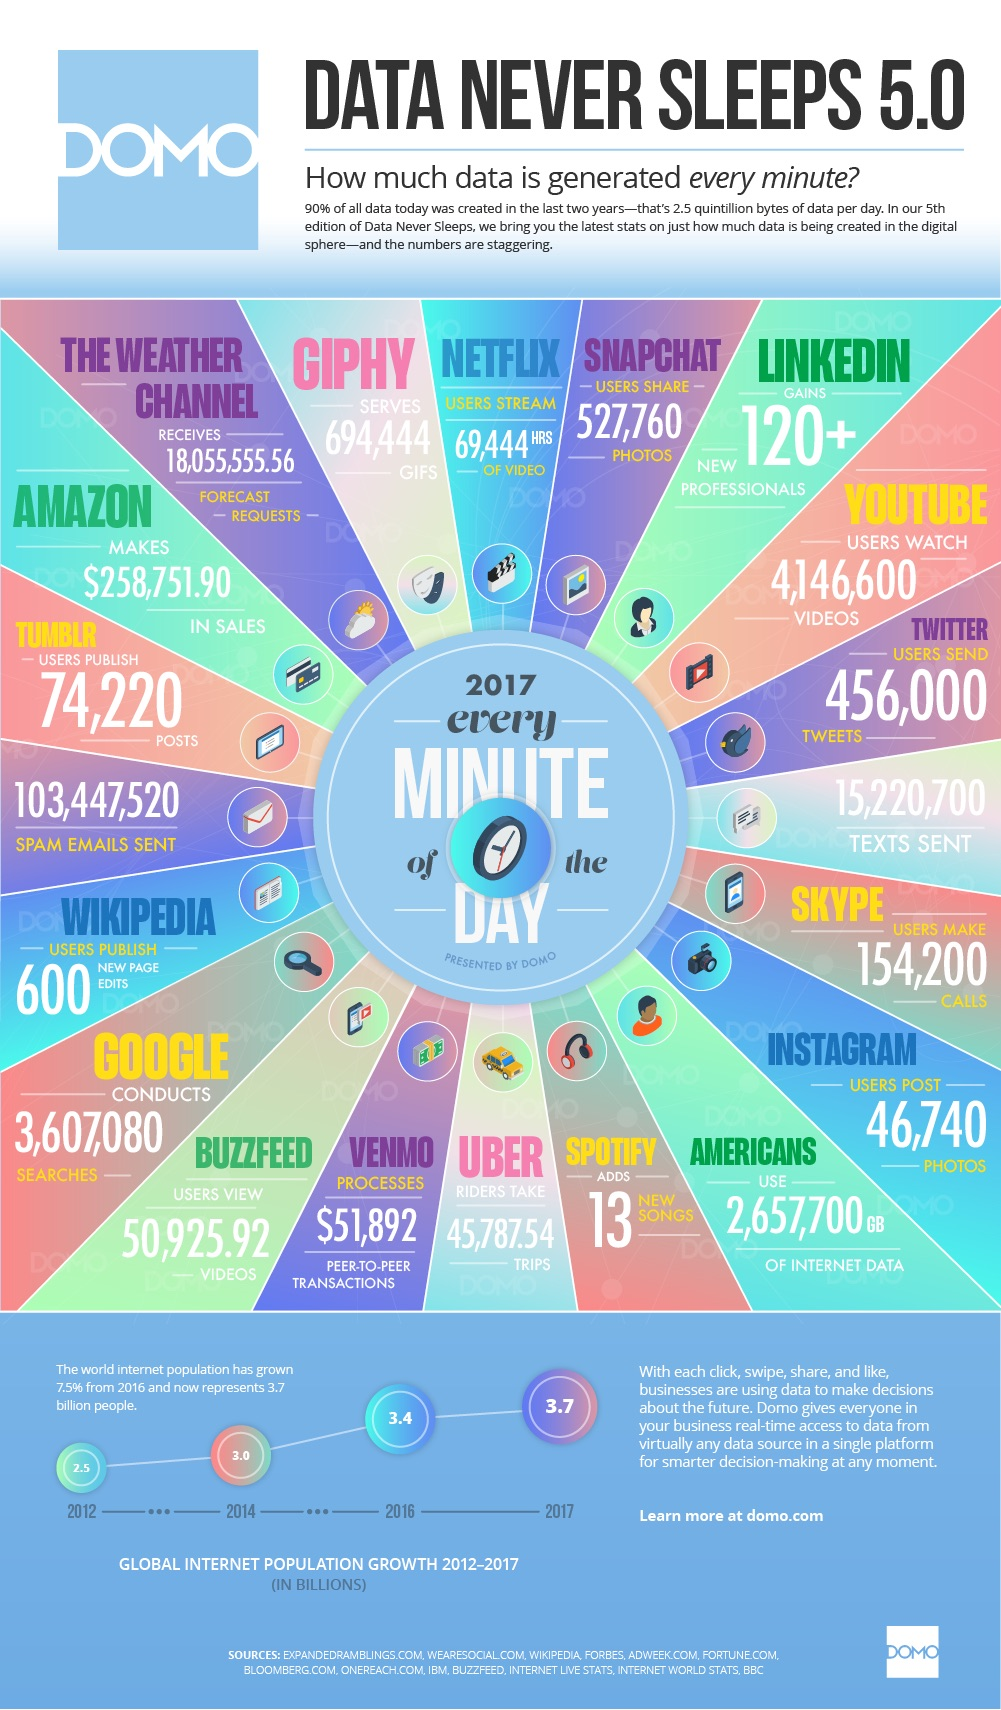
\includegraphics[width = 13 cm]{./viz/ext/dataeachday2017.jpg}
\end{figure}

\newpage
%=========================================
\subsection{Stages of Data Exploration}
%=========================================
\begin{HIGHLIGHT}
\par\noindent{
The various stages of data exploration can be classified into the following:
\begin{enumerate}
  \item Accessing Data
  \item Transforming Data
  \item Generating Summaries of the Data
  \item Making Predictions on the Data
  \item Communicating Findings
\end{enumerate}
}
\end{HIGHLIGHT}

\begin{DIY}{Think}
Which \emph{Stages of Data Exploration} did you apply while exploring the dataset in exercise1.csv
\end{DIY}

%=========================================
\subsection{Challenges of Data Exploration}
%=========================================
%=========================================
\subsubsection{Misuse, Misinterpretation and Bias}
%=========================================

%=========================================
\subsubsection{Data Preparation and Cleaning}
%=========================================

%=========================================
\subsubsection{Missing Data and Data Errors}
%=========================================

%=========================================
\subsubsection{Statistical Error}
%=========================================

%=========================================
\subsection{The Geometry of Data}
%=========================================
\newpage
%=========================================
\subsection{Software for Data Exploration}
%=========================================
\begin{HIGHLIGHT}
\par\noindent{
{\centering\textbf{\emph{\Large ``Trustworthy, Flexible and Efficient Software: The Prime Directives''}} \\}
\vspace{\baselineskip}
\noindent The task of data exploration requires a tool that allows a user to ask meaningful questions about their applications quickly and flexibly. A wide range of techniques is needed to facilitate stages 1-4 of data exploration thereby requiring the data exploration tool to be flexible. Moreover, the tool should be able to provide answers to the questions asked ``\emph{within an acceptable timeframe}''. The \textbf{3V's}, and the questions that are posed on the data, require complex transformations and computations on the data, whose correctness cannot be often verified by direct observation of the results in stage 5. Therefore, it is imperative that the underlying implementations of the transformations and computaions (which is often \textbf{\emph{encapsulated}}) are correct.
}
\end{HIGHLIGHT}

\begin{DIY}{Think}
How does Microsoft Excel provide \textbf{\emph{Abstraction via Encapsulation}}. Think of an example where the trustworthiness comes into play.
\end{DIY}

\begin{DIY}{Warning}
It is extremely hard to achieve \emph{trustworthiness}, \emph{flexibility} and \emph{efficiency} at the same time. As you go ahead in the course try to identify trade-offs between the three directives in R.  
\end{DIY}


\newpage

% !Rnw root = Introduction.Rnw
%==========================
\section{Why R?}
%==========================
\noindent Before delving into the question of \emph{why R?}, let us first take a look at how R fares with respect to to its competitors.The following two plots show the results of two surveys conducted in the year 2017. The first plot shows the result of a similar survey, conducted worlwide, by Kaggle.The second survey was conducted by O'Rielly in Europe and shows the popularity of different tools among data analysts/scientists.As is evident from both plots, R is a highly popular tool among data analysts/scientists.

    % Figure to demonstrate popularity of R in Kaggle surveys
    \begin{figure}[ht] % Figure to demonstrate popularity of R in O'Rielly surveys
      \centering
      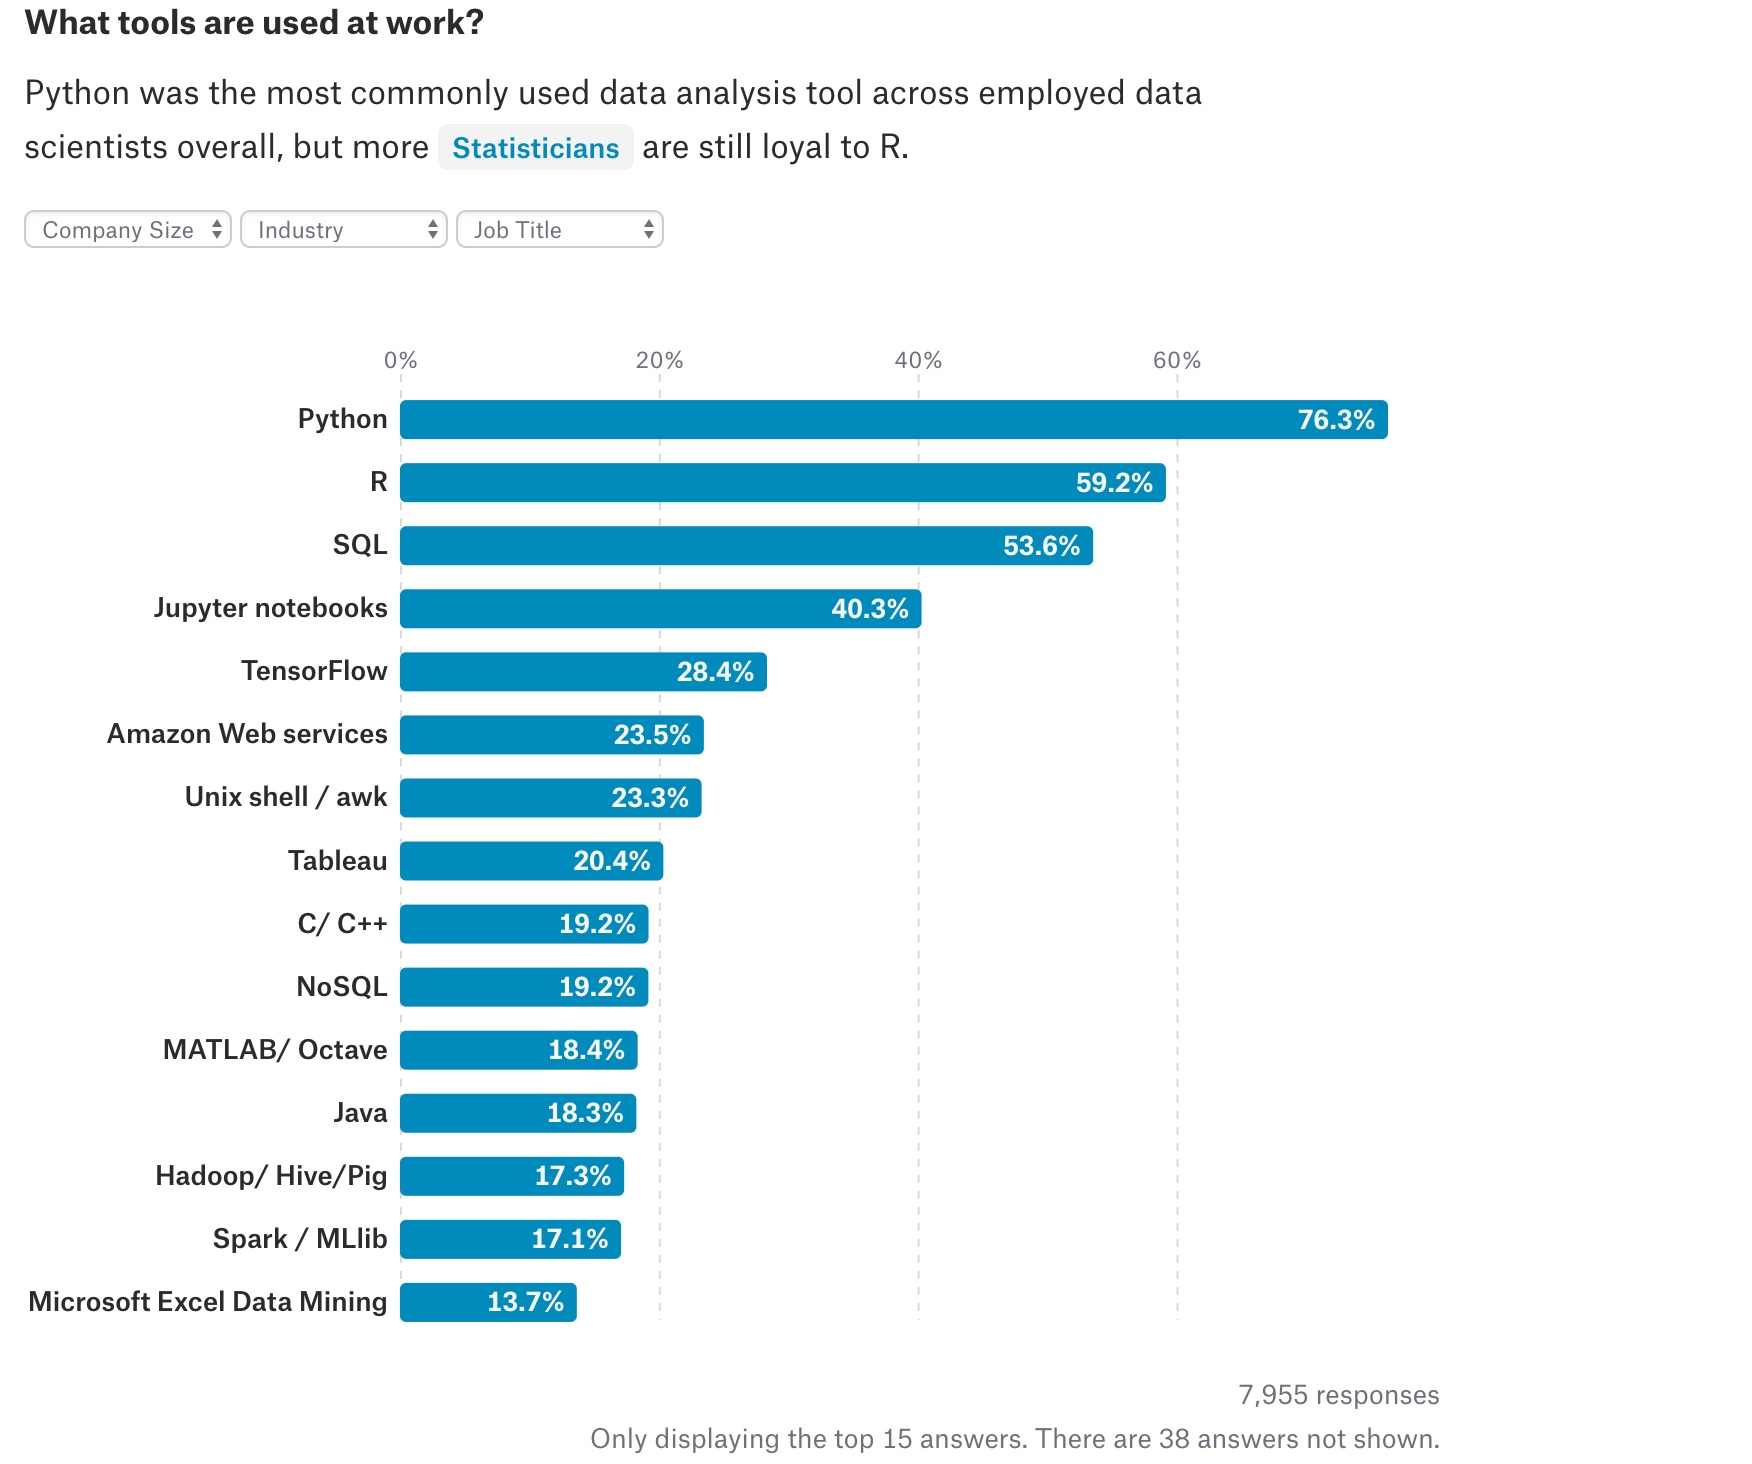
\includegraphics[width = 15 cm]{./viz/ext/Kaggle_DS_Tools_Survey.jpeg}
    \end{figure}

    \begin{figure}[ht] % Figure to demonstrate popularity of R in O'Rielly surveys
      \centering
      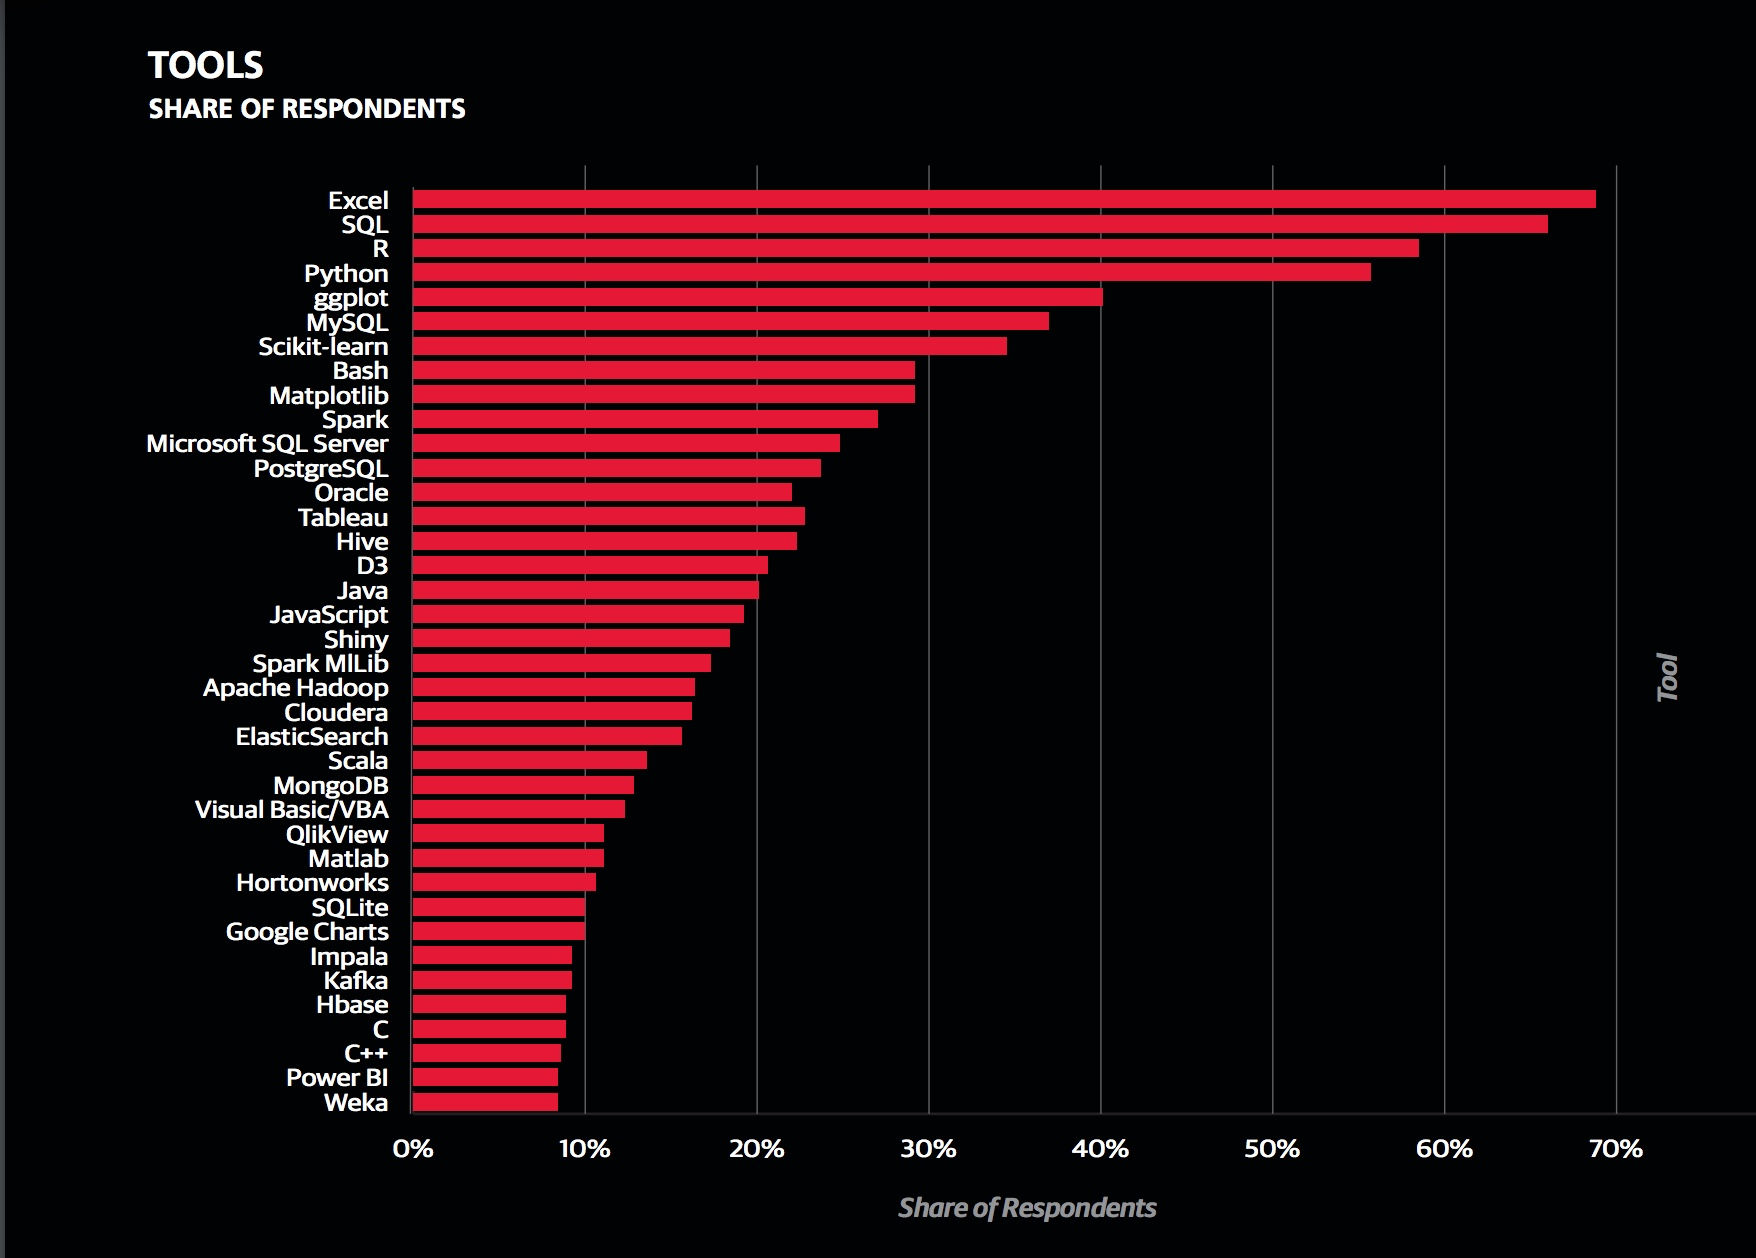
\includegraphics[width = 15 cm]{./viz/ext/OR_DS_Tools_Survey.jpeg}
    \end{figure}
    
\begin{DIY}{Think}
\emph{Think like an Analyst:} Criticize the plots in terms of their inadequacy to provide the complete information. Argue, why and how would this lead to drawing of incorrect conclusions. 
\end{DIY}

\begin{DIY}{Homework}
Read the reports
\begin{enumerate}
  \item \textbf{``Eupopean Data Science Salary Survey''} published by O'REILLY in 2017
  \item \textbf{``The State of Data Science \& Machine Learning''} published by Kaggle in 2017
\end{enumerate}
and get yourself acquainted with \emph{stage 5} of the data exploration process.
\end{DIY}

%================================  
\subsection{A Brief History of R}
%================================
\textcolor{yellow}{TODO}
%================================
\subsection{Concepts for Programming with R}
%================================
%================================
\subsubsection{Functional Programming}
%================================
\begin{HIGHLIGHT}
\par\noindent{
Software in R is written in a \emph{functional style} that 
emphasizes on \emph{encapsulating computations via functions} thereby allowing the programmer to create \emph{abstractions by separating behaviour from implementation}.}
\end{HIGHLIGHT}

\begin{DIY}{Think}
If you are given a set of $N$ numbers whose average needs to be computed, think about how would the functional programming approach allow you to achieve abstraction and what would be its benefit?
\emph{Hint:} Think about how would the computation of average differ when $N$ numbers are given in one go (\textbf{\emph{batched input}}) as opposed to when you get every number one after the other (\textbf{\emph{streaming input}})
\end{DIY}

%================================
\subsubsection{Classes and Methods}
%================================
\begin{HIGHLIGHT}
\par\noindent{
\emph{``Functions in R return objects'}'. Therefore any kind of \textbf{\emph{data in R is always an object}}. While functions facilitate abstraction by encapsulating implementation of computation, \emph{classes encapsulate objects}. \emph{Methods in R knit together functions and classes}.   
}
\end{HIGHLIGHT}
%================================
\subsubsection{Data Frames}
%================================
\begin{HIGHLIGHT}
\par\noindent{
A \emph{data frame} is organization of data as observations (rows) and attributes (columns). Data frames are one of the predominant data structures in R. Moreover, they are synonymous with the tabular rebresentation of data as is found in spreadsheets and relational database systems. Such similarity in representation of data enables seamless integration between R and most spreadsheets and RDBMS systems. 
}
\end{HIGHLIGHT}
%================================
\subsubsection{Ecosystem}
%================================
\begin{HIGHLIGHT}
\par\noindent{
R is an open-source software, thereby providing access to source code sufficient to generate a working version of the software. R is distributed under a version of GPL (Gnu Public License). An effect of this is that R has a thriving community of contributors and active users. Users, seek out existing implementation of data analysis/modeling techniques from a repository caled \textbf{\emph{CRAN}} (\textcolor{cyan}{\url{https://cran.r-project.org/}}). When they do not find an existing implementation that suits their needs, they create their own implementations, \emph{package} these implementations and contribute them back to CRAN. As a result of this CRAN today boasts a total of 12000+ packages. Please see the plot below that shows the growth in number of CRAN packages over time. This has resulted in R being unparalled in the number of options it provides for data analysis. Moreover, R is the primary tool used for statistical research (and has been so for 20 years). Therefore, when new methods are developed, they are not just published as a paper - they are also published as an R package. This means R is always on the cutting edge of new technologies. Furthermore, R was designed as an interface language - a means to present a consistent language interface for algorithms written in other languages. Many packages work by providing R language bindings to other open-source software, making R a convenient hub for all kinds of algorithms and methods.     
}
\end{HIGHLIGHT}

\begin{figure}[ht] % Figure to demonstrate growth in number of CRAN packages over time
      \centering
      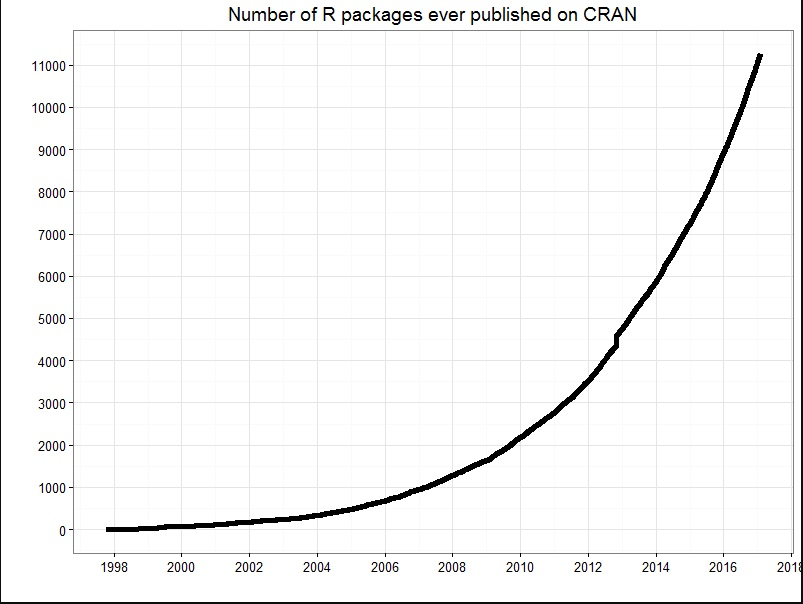
\includegraphics[width = 10 cm]{./viz/ext/numberofCRANpackages_over_Time.jpeg}
    \end{figure}

\begin{DIY}{Think}
Did you notice the sudden discontinuity in the curve around the year 2013? Can you think of what might have caused this?
\end{DIY}

\begin{DIY}{Think}
Argue \textbf{\emph{Why R}} statisfies \emph{the prime directives} and should therefore be our tool of choice for our mission of data exploration
\end{DIY}
    
\section{RStudio}

\begin{HIGHLIGHT}
\par\noindent{
\begin{DIY}{Homework}
Watch the video on \\
\textcolor{cyan}{\url{https://www.rstudio.com/resources/webinars/rstudio-essentials-webinar-series-part-1/}}\\
and install R and RStudio on the computer that you will be accessing during the sessions.
\end{DIY}
}
\end{HIGHLIGHT}

\begin{DIY}{Warning}
\textcolor{red}{It is important that the participants have R and RStudio installed on their computers before Session 1.}
\end{DIY}

\begin{DIY}{Homework}
Download the RStudio IDE Cheat Sheet and use it as a reference while working with RStudio. In order to download the Cheat Sheet, \emph{Open RStudio $>$ Go to  Help Menu $>$ Cheatsheets $>$ RStudio IDE Cheat Sheet}
\end{DIY}


% !Rnw root = Introduction.Rnw
%===============================
\section{Using R}
%===============================
%===============================
\subsection{An Interactive Session}
%===============================
\begin{HIGHLIGHT}
\par\noindent{
R is an \emph{interactive} environment, wherein the users gets immediate feedback (\emph{results}) for their instructions (\emph{expressions}). This is in contrast to programming languages like C++ or Java wherein a set of instructions (the program) has to be created and compiled before the results can be generated.In R, the interaction between the user and the system constitutes an \emph{R Session}. During an R session, the user provides \emph{expressions} to R for doing computations, displaying results, and creating objects for further use. R, first evaluates the expressions for its syntactic correctness and then performs the task, as specified by the expression. We will examine some basic expressions in the next section.     
}
\end{HIGHLIGHT}

\begin{HIGHLIGHT}
\par\noindent{
R, like Python, MATLAB etc is a \emph{dynamically typed language} which means that you won't have to define the type of the variable (which stores your data). As a result, the user can only focus on the \emph{data stored by the variable} rather than having to worry about \emph{how the data is stored in the variable}. This is in stark contrast to \emph{statically typed languages} like C++ and Java.      
}
\end{HIGHLIGHT}

\begin{DIY}{Think}
How does a R \emph{data frame} exemplify the \emph{dynamic typing} feature of R?
\end{DIY}
    
\begin{DIY}{Warning}
The dynamic typing feature of R  provides great flexibility but at what cost?
\end{DIY}



% !Rnw root = UsingR.Rnw
%==================================  
\subsection{Basic Expressions in R}
%==================================  
At the \emph{console}, the user finds the \textbf{$>$} prompt where the user responds by typing and expression. Hereon, in this section every expression/set of expressions is mentioned in the gray box and is to be issued at the $>$ prompt in the console. Moreover, following the motto of this course ``learn by doing``, the reader is strongly encouraged to try out each of these expressions and \emph{read the corresponding help manual for each expression}. As is evident from the examples shown in this section, expressions are predominantly \textbf{\emph{function calls with a set of arguments}}.

\begin{HIGHLIGHT}
\par\noindent{
Objects are the center of computations in R, along with the function calls that create and use those objects.
}
\end{HIGHLIGHT}

\begin{DIY}{Think}
What are objects in R? Why are functions and objects dual to each other? 
\end{DIY}

%==================================  
\subsubsection{Data sets in R}
%==================================  
\noindent R comes packaged with a list of data sets which can be viewed with the following command: 
\begin{knitrout}
\definecolor{shadecolor}{rgb}{0.969, 0.969, 0.969}\color{fgcolor}\begin{kframe}
\begin{alltt}
\hlkwd{library}\hlstd{(}\hlkwc{help} \hlstd{=} \hlstr{"datasets"}\hlstd{)}
\end{alltt}
\end{kframe}
\end{knitrout}
\noindent These data sets are a great starting point for new comers to try out different R expressions on, and getting your hands dirty. 
%==================================  
\subsubsection{Want Help?: Use the ``\textbf{?}'' operator}
%==================================  
\noindent The \textbf{?} operator displays help for the topic that follows it.
\begin{knitrout}
\definecolor{shadecolor}{rgb}{0.969, 0.969, 0.969}\color{fgcolor}\begin{kframe}
\begin{alltt}
\hlopt{?}\hlstd{data.frame}
\end{alltt}
\end{kframe}
\end{knitrout}

\begin{DIY}{Think}
What is an operator? What other operators can you think of? 
\end{DIY}

\noindent Another way of displaying documentation for a topic is by calling the $help()$ function with the topic as its argument. 
\begin{knitrout}
\definecolor{shadecolor}{rgb}{0.969, 0.969, 0.969}\color{fgcolor}\begin{kframe}
\begin{alltt}
\hlkwd{help}\hlstd{(}\hlstr{"data.frame"}\hlstd{)}
\end{alltt}
\end{kframe}
\end{knitrout}
%==================================  
\subsubsection{Want to view a dataset?: Use the $View()$ function}
%==================================  
\noindent The $View()$ function can be used to see the contents of a data set wherein the argument to the function is the object that contains the data.
\begin{knitrout}
\definecolor{shadecolor}{rgb}{0.969, 0.969, 0.969}\color{fgcolor}\begin{kframe}
\begin{alltt}
\hlkwd{View}\hlstd{(iris)}
\end{alltt}
\end{kframe}
\end{knitrout}
%==================================  
\subsubsection{Want to get type of an object?: Use the $class()$ function}
%==================================  
\noindent We can get the type of an R object by using the $class()$ function. This is synonymous to using the $DESC()$ function in your SQL query  
\begin{knitrout}
\definecolor{shadecolor}{rgb}{0.969, 0.969, 0.969}\color{fgcolor}\begin{kframe}
\begin{alltt}
\hlkwd{class}\hlstd{(iris)}
\end{alltt}
\begin{verbatim}
## [1] "data.frame"
\end{verbatim}
\end{kframe}
\end{knitrout}
%==================================  
\subsubsection{Want to count rows and columns?: Use the $dim()$ function}
%==================================  
\noindent For objects that have a tabular structure, the $dim()$ function enalbes us to get the number of rows (observations) and number of columns (attributes)  
\begin{knitrout}
\definecolor{shadecolor}{rgb}{0.969, 0.969, 0.969}\color{fgcolor}\begin{kframe}
\begin{alltt}
\hlkwd{dim}\hlstd{(iris)}
\end{alltt}
\begin{verbatim}
## [1] 150   5
\end{verbatim}
\end{kframe}
\end{knitrout}
\noindent Now,try:
\begin{knitrout}
\definecolor{shadecolor}{rgb}{0.969, 0.969, 0.969}\color{fgcolor}\begin{kframe}
\begin{alltt}
\hlkwd{class}\hlstd{(}\hlkwd{dim}\hlstd{(iris))}
\end{alltt}
\begin{verbatim}
## [1] "integer"
\end{verbatim}
\end{kframe}
\end{knitrout}
\begin{DIY}{Think}
Do you see the difference in result when iris is passed as an argument to $class()$ v/s when $dim(iris)$ is passed as an argument to $class()$. Think about what does the output signify?   
\end{DIY}

\begin{DIY}{Think}
Did you notice how $class()$ takes a data.frame as an argument in one case while takes $dim(iris)$ in another. Relate this observation to the ideas of objects and encalsulation that we have discussed until now.   
\end{DIY}

\begin{DIY}{Think}
What other data types exist in R?   
\end{DIY}
%==================================  
\subsubsection{Want to get an Element of an Array?: Use the [] operator}
%==================================  
\noindent Objects, for which the $class()$ function returns a 'numeric' or 'integer' type are essentially an \emph{array of numbers}, elements of which, can be accessed using the \textbf{[]} operator     
\begin{knitrout}
\definecolor{shadecolor}{rgb}{0.969, 0.969, 0.969}\color{fgcolor}\begin{kframe}
\begin{alltt}
\hlkwd{dim}\hlstd{(iris)[}\hlnum{1}\hlstd{]}
\end{alltt}
\begin{verbatim}
## [1] 150
\end{verbatim}
\begin{alltt}
\hlkwd{dim}\hlstd{(iris)[}\hlnum{2}\hlstd{]}
\end{alltt}
\begin{verbatim}
## [1] 5
\end{verbatim}
\end{kframe}
\end{knitrout}

\begin{DIY}{Think}
What do you observe when you try $dim(iris)$[0] ? Explain your observation. 
\end{DIY}
%==================================  
\subsubsection{Want to Assign a Value?: Use the $<-$ operator}
%==================================  
\noindent A number of times we will need to assign the object returned by a function to another object. This is done using the $<-$ operator 
\begin{knitrout}
\definecolor{shadecolor}{rgb}{0.969, 0.969, 0.969}\color{fgcolor}\begin{kframe}
\begin{alltt}
\hlstd{result} \hlkwb{<-} \hlkwd{dim}\hlstd{(iris)[}\hlnum{1}\hlstd{]}
\hlstd{result}
\end{alltt}
\begin{verbatim}
## [1] 150
\end{verbatim}
\end{kframe}
\end{knitrout}

\begin{DIY}{Think}
Explain how the \emph{dynamic typing} feature of R is evident here. 
\end{DIY}
%==================================  
\subsubsection{Want to View a Column?: Use the \textbf{\$} operator}
%==================================  
\noindent Attributes of an R object can be accessed by the \textbf{\$} operator. This operator is synonymous to selecting a column in a spreadsheet or a database table.
\begin{knitrout}
\definecolor{shadecolor}{rgb}{0.969, 0.969, 0.969}\color{fgcolor}\begin{kframe}
\begin{alltt}
\hlstd{resut}\hlkwb{<-}\hlstd{iris}\hlopt{$}\hlstd{Sepal.Length}
\end{alltt}
\end{kframe}
\end{knitrout}
%==================================  
\subsubsection{Want to Count Number of elements?: Use the $length()$ function}
%==================================  
\noindent Once we have selected an attribute, we can count the number of elements in it using the $length()$  function and passing the attribute object as an argument to it. This function is synonymous to using $COUNT*$ in your SQL query.
\begin{knitrout}
\definecolor{shadecolor}{rgb}{0.969, 0.969, 0.969}\color{fgcolor}\begin{kframe}
\begin{alltt}
\hlkwd{length}\hlstd{(iris}\hlopt{$}\hlstd{Sepal.Length)}
\end{alltt}
\begin{verbatim}
## [1] 150
\end{verbatim}
\end{kframe}
\end{knitrout}
%==================================  
\subsubsection{Want to Get Distinct Elements?: Use the $unique()$ function}
%==================================  
\noindent We can get the list of unique elements belonging to an attribute by using the $unique$ function. This function is synonymous to using the $DISTINCT()$ function in your SQL query  
\begin{knitrout}
\definecolor{shadecolor}{rgb}{0.969, 0.969, 0.969}\color{fgcolor}\begin{kframe}
\begin{alltt}
\hlkwd{unique}\hlstd{(iris}\hlopt{$}\hlstd{Sepal.Length)}
\end{alltt}
\end{kframe}
\end{knitrout}
%==================================  
\subsubsection{Want to Get Sum?: Use the $sum()$ function}
%==================================  
\noindent Elements of a numeric vector can be easily summmed up by passing it as an argument to the $sum()$ function
\begin{knitrout}
\definecolor{shadecolor}{rgb}{0.969, 0.969, 0.969}\color{fgcolor}\begin{kframe}
\begin{alltt}
\hlkwd{sum}\hlstd{(iris}\hlopt{$}\hlstd{Sepal.Length)}
\end{alltt}
\begin{verbatim}
## [1] 876.5
\end{verbatim}
\end{kframe}
\end{knitrout}
%==================================  
\subsubsection{Want to Get Cumulative Sum?: Use the $cumsum()$ function}
%==================================  
\noindent The cumulative sum of elements in a numeric vector can be computed by passing it as an argument to the $cumsum()$ function
\begin{knitrout}
\definecolor{shadecolor}{rgb}{0.969, 0.969, 0.969}\color{fgcolor}\begin{kframe}
\begin{alltt}
\hlkwd{cumsum}\hlstd{(iris}\hlopt{$}\hlstd{Sepal.Length)}
\end{alltt}
\end{kframe}
\end{knitrout}
%==================================  
\subsubsection{Want to Creat a Histogram?: Use the $hist()$ function}
%==================================  
\noindent A histogram which plots the number of occurences of distinct elements (\textbf{\emph{discrete variables}}) in the attribute or number of occurences of distinct intervals (\textbf{\emph{continuous variables}}) in the attribute.
\begin{knitrout}
\definecolor{shadecolor}{rgb}{0.969, 0.969, 0.969}\color{fgcolor}\begin{kframe}
\begin{alltt}
\hlkwd{hist}\hlstd{(iris}\hlopt{$}\hlstd{Sepal.Length)}
\end{alltt}
\end{kframe}
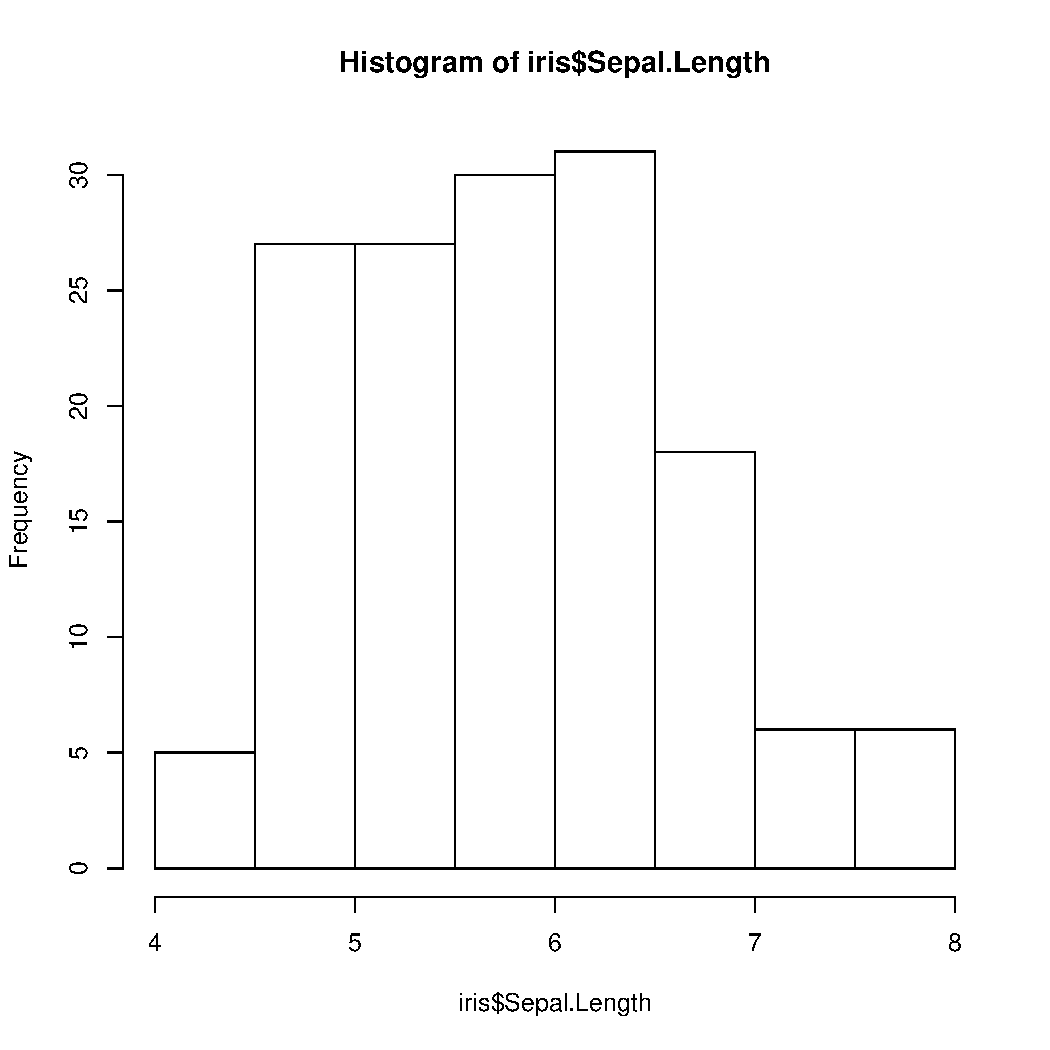
\includegraphics[width=\maxwidth]{figure/hist-1} 

\end{knitrout}

\begin{DIY}{Think}
Is the argument passed to $hist()$ a \emph{discrete attribute} or a \emph{continuous attribute}? Explain your choice.
\end{DIY}

\begin{DIY}{Think}
Change the histogram plot to show normalized frequencies
\end{DIY}
%==================================  
\subsubsection{Want to Get Part of an Array?: Use the [] operator for sub-setting}
%==================================  
\begin{knitrout}
\definecolor{shadecolor}{rgb}{0.969, 0.969, 0.969}\color{fgcolor}\begin{kframe}
\begin{alltt}
\hlstd{iris}\hlopt{$}\hlstd{Sepal.Length[}\hlnum{1}\hlopt{:}\hlnum{10}\hlstd{]}
\end{alltt}
\begin{verbatim}
##  [1] 5.1 4.9 4.7 4.6 5.0 5.4 4.6 5.0 4.4 4.9
\end{verbatim}
\end{kframe}
\end{knitrout}

\begin{DIY}{Homework}
Find the sum of the first 10 and last 10 elements of the numeric array.
\end{DIY}
%==================================  
\subsubsection{Want to Create an XY Plot?: Use the $plot()$ function}
%==================================  
\noindent The plot function takes two numeric arrays as arguments and treats each pair of values in the in the arguments as $(X,Y$ coordinates, thereby producing a scatter plot 
\begin{knitrout}
\definecolor{shadecolor}{rgb}{0.969, 0.969, 0.969}\color{fgcolor}\begin{kframe}
\begin{alltt}
\hlkwd{plot}\hlstd{(cars}\hlopt{$}\hlstd{speed,cars}\hlopt{$}\hlstd{dist)}
\end{alltt}
\end{kframe}
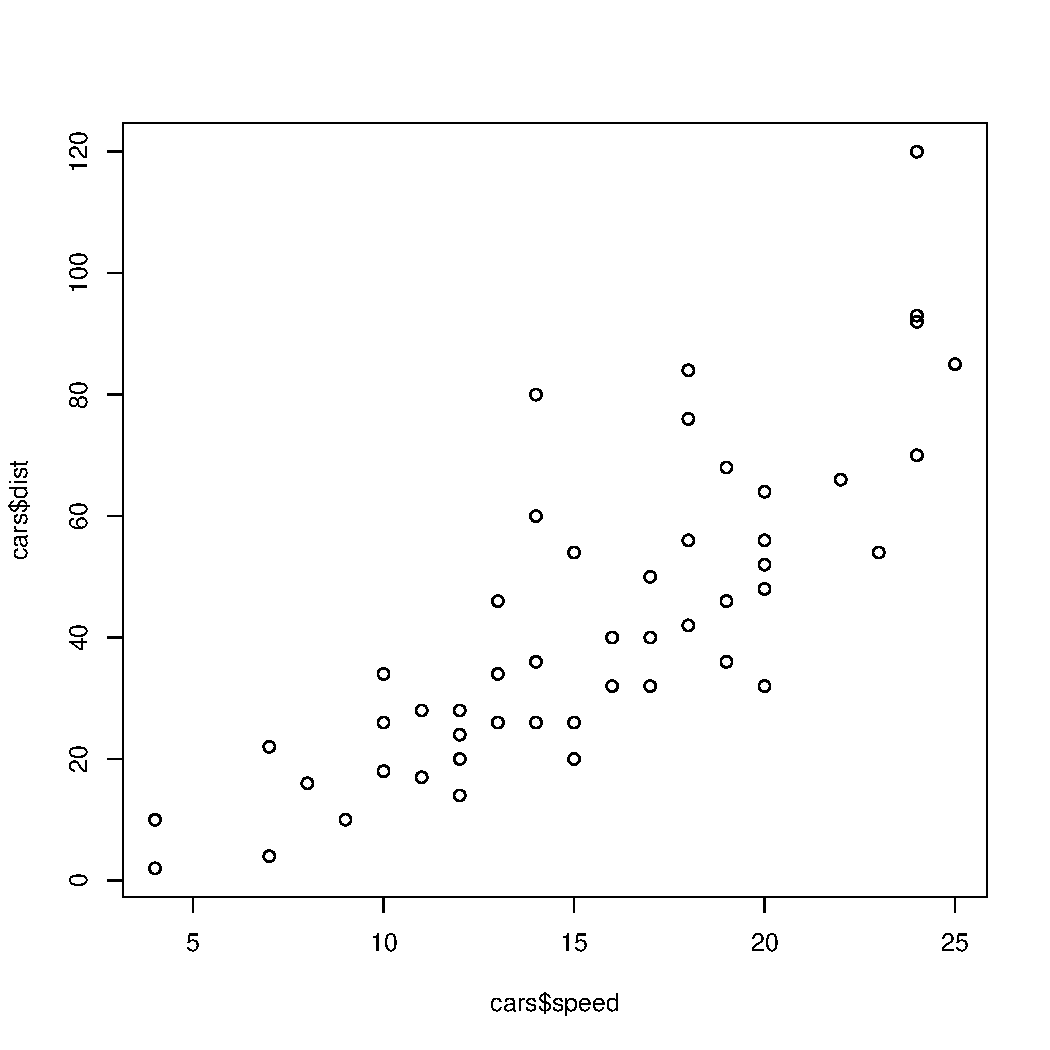
\includegraphics[width=\maxwidth]{figure/plot-1} 

\end{knitrout}

\begin{DIY}{Think}
Can you \emph{explain} the plot that you see above?
\end{DIY}

\begin{DIY}{Think}
Change the markers in the plot from circles to crosses. Moreover change the of the markers
\end{DIY}

\begin{DIY}{Think}
What will you get when you pass a data frame with three attributes as an argument to the $plot()$ func function
\end{DIY}

\begin{DIY}{Homework}
Pick a dataset from the list of available datasets and \emph{explore it} using the \emph{R expressions} you have just learnt.
\end{DIY}
%===============================
\subsection{Input/Output(I/O) with External Sources}
%===============================
\begin{HIGHLIGHT}
\par\noindent{
Reading in data from files like ``\textbf{.txt}'',``\textbf{.csv}'' and ``\textbf{.xls}'' into the R environment has been greatly simplified by RStudio. Just goto  Environment tab $->$ Import Dataset  and select the file type from which you want to import the data (for \emph{.txt} and  \emph{.csv} files choose the ``From CSV...'' option while for excel sheets choose ``From Excel..'' option). A new window will open up with a set of options that will guide you to import your data in R.        
}
R also provides a set of functions for reading and writing data. An inquisitive reader can read about them in \textcolor{cyan}{\url{https://www.datacamp.com/community/tutorials/r-tutorial-read-excel-into-r}}
\end{HIGHLIGHT}

\begin{DIY}{Think}
Though RStudio has simplified the process of reading in data by providing a GUI, it hasn't provided any machanism for writing data out of the R environment. What do you think this is the reason for this?  
\end{DIY}

\begin{DIY}{Homework}
Do the following
\begin{enumerate}
  \item Remove the headers from exercise1.csv and try importing it into the R environment. What do you observe?
  \item Replace exercise1.csv as exercise1.tsv (i.e change the delimiter between attributes from comma to tab) and try importing it into the R environment.
\end{enumerate}
\end{DIY}
%===============================
\subsubsection{IO with Relational Database Management Systems(RDBMS)}
%===============================
%=============================
\begin{figure}[ht]
 \centering
    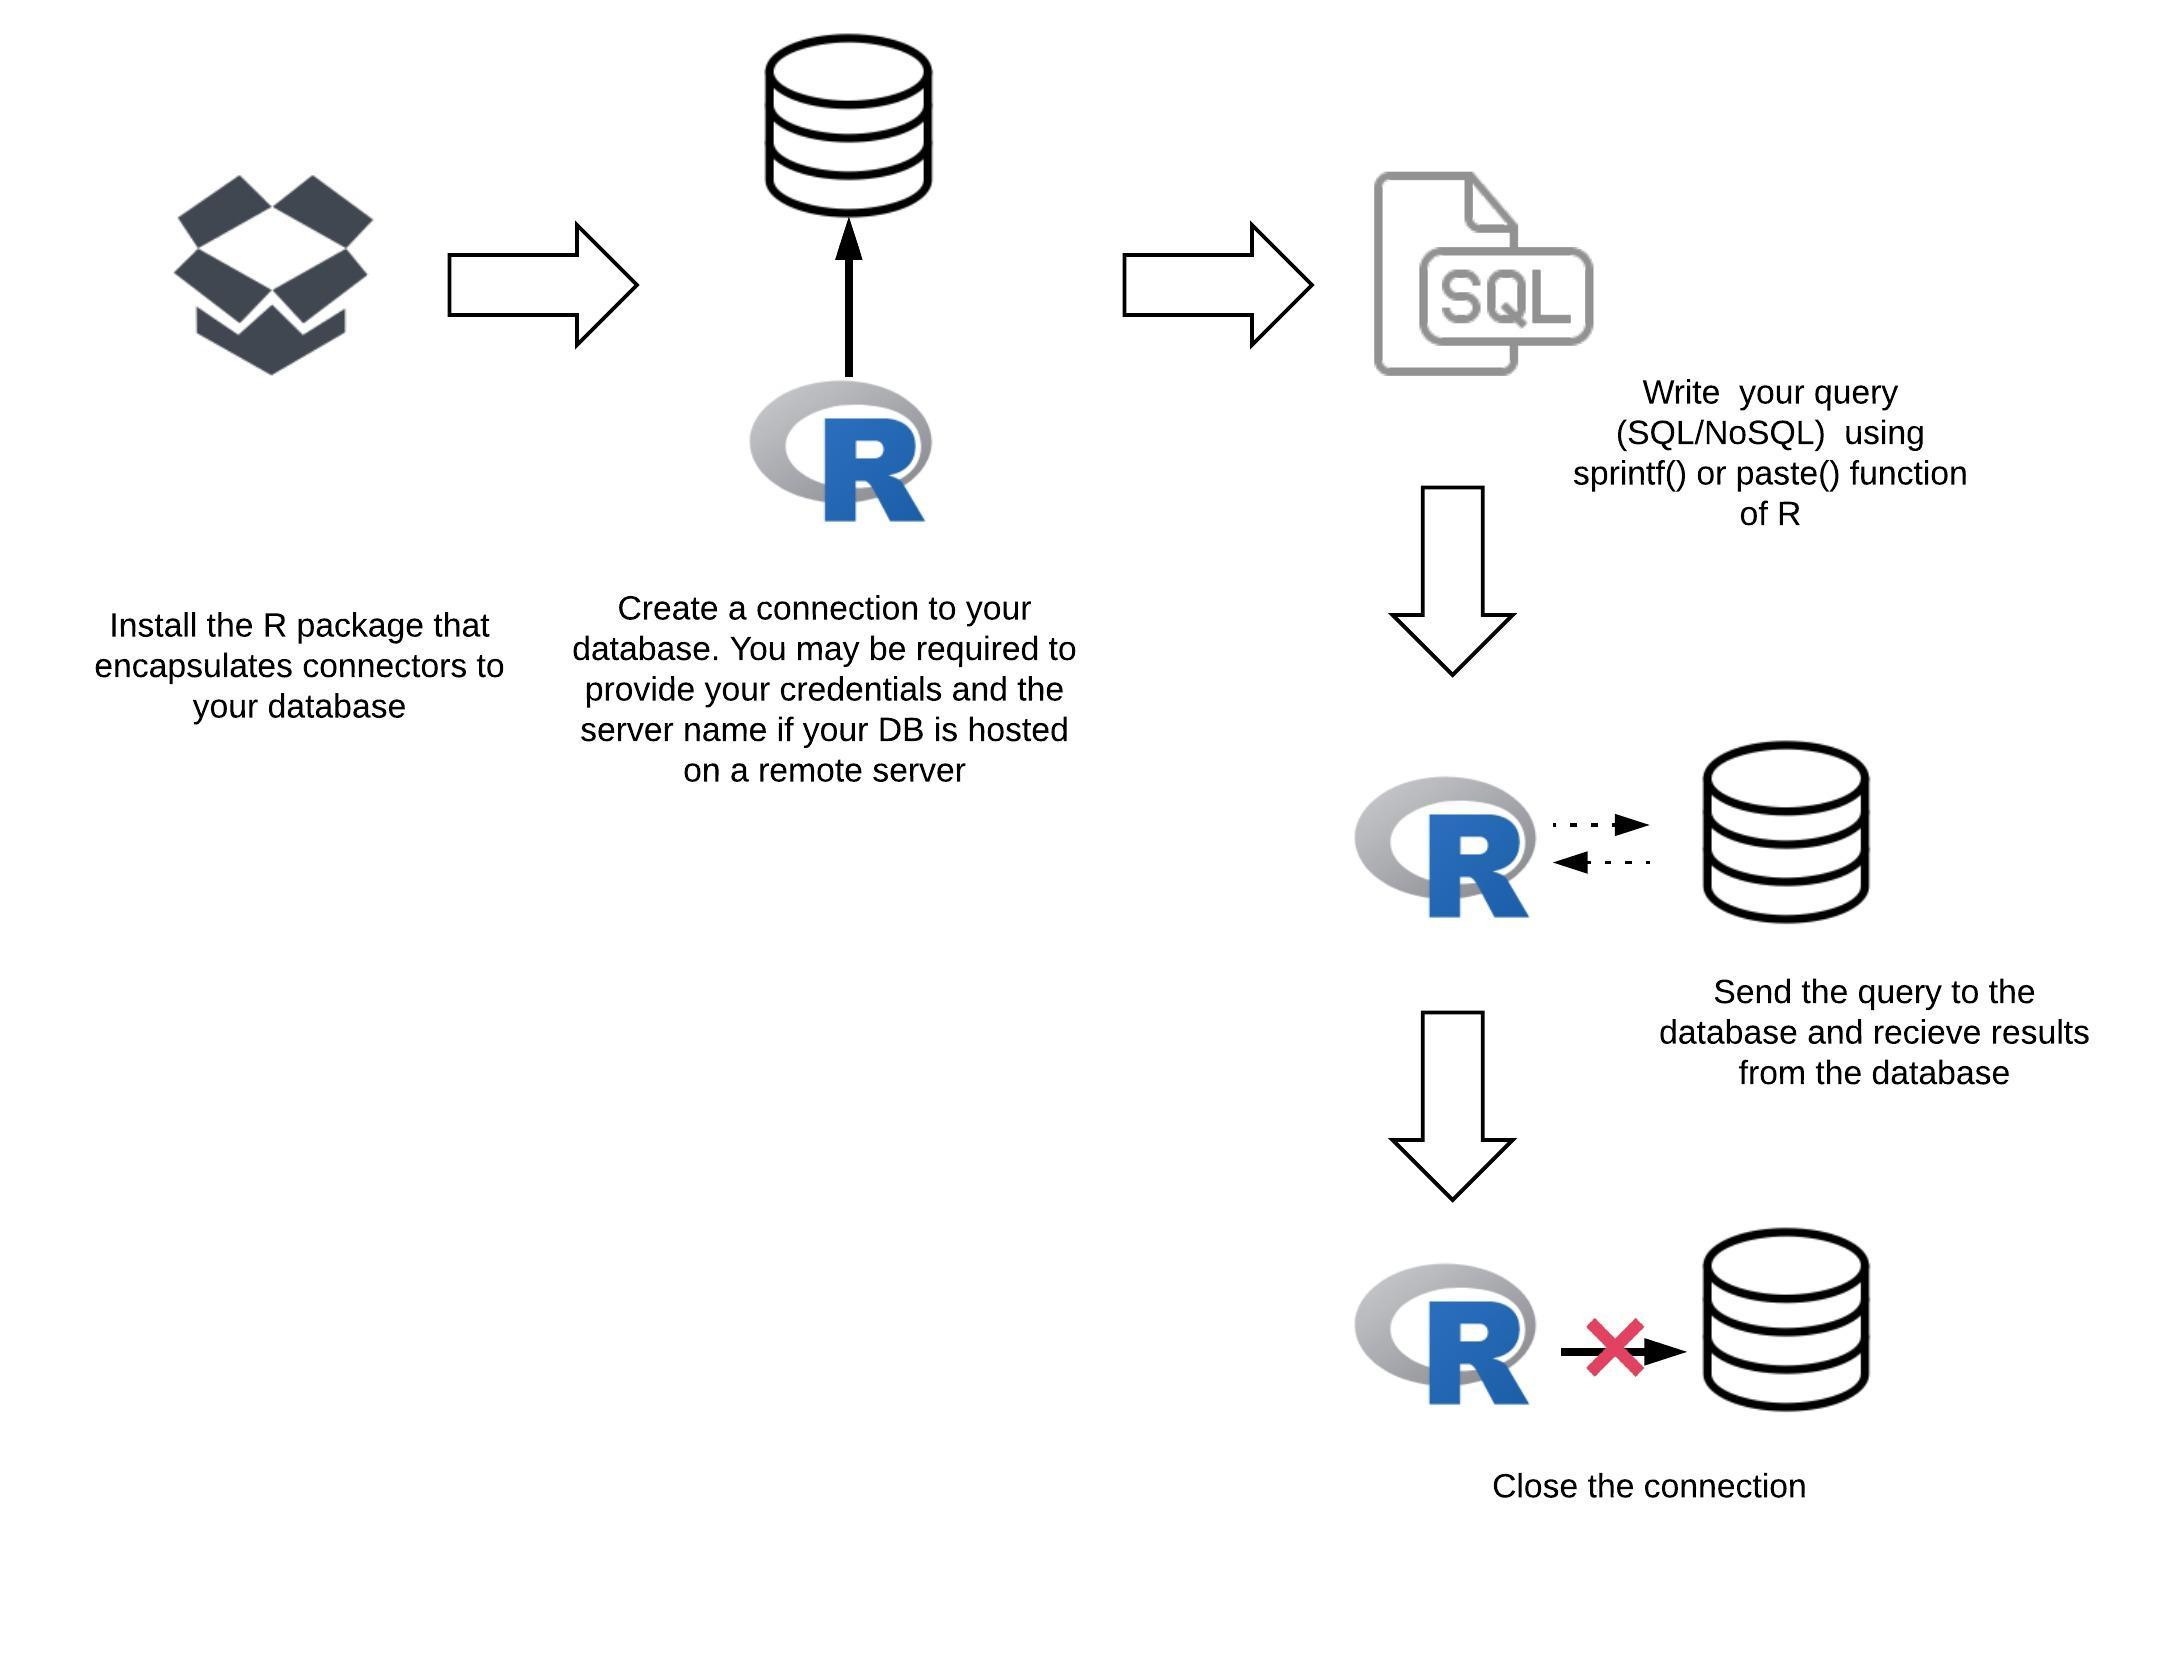
\includegraphics[width = 15 cm]{./viz/ext/IO_R_RDBMS.jpeg}
\end{figure}
\begin{HIGHLIGHT}
A large number of different databases exist in the market and each of them has is its own way of setting up and managing connections with client applications. These low level connection details are encapsulated by R packages and the user only has to be aware of of an abstract view as shown in the schematic. Details of R packages for connecting to some of the popular databases can be found in the following links:
\begin{itemize}
  \item How to Connect to an Oracle Database:
  
  \textcolor{cyan}{\url {http://rprogramming.net/connect-to-database-in-r/}}
  \item How to Connect to a MySQL Database:
  
  \textcolor{cyan}{\url {https://www.r-bloggers.com/mysql-and-r/}}
  \item How to Connect to MongoDB: 
  
  \textcolor{cyan}{\url {https://www.r-bloggers.com/r-and-mongodb/}}
\end{itemize}

\end{HIGHLIGHT}
